\chapter{Background}
In questo capitolo verrà descritta la tecnologia alla base di Bitcoin. Particolare attenzione verrà data alla blockchain, la struttura dati che costituisce il libro contabile dove vengono registrate le transazioni, al funzionamento delle transazioni, agli indirizzi per esporre infine la problematica relativa all'anonimato degli utenti di Bitcoin. 
\section{Funzioni hash}
Il meccanismo utilizzato da Bitcoin per garatnire l'integrità e l'immutabilità della  blockchain sono le funzioni hash.

Una funzione hash $f$: X $\longrightarrow$ Y è una funzione matematica avente come dominio X e codominio Y, insiemi finiti tali che $|X| >> |Y |$.

Tale funzione prende in input elementi di X di lunghezza qualsiasi e produce in output, a prescindere dalla lunghezza dell’input, stringhe binarie di dimensione fissa, i cosiddetti fingerprint, chiamati anche immagini hash o semplicemente hash.

Una proprietà fondamentale delle funzioni hash è relativa al tempo necessario al loro calcolo: devono essere calcolate efficientemente, ossia a fronte di un input di $m$ bit, la complessità computazionale per produrne il fingerprint deve essere $O(m)$, lineare o comunque polinomiale nei bit su cui è rappresentato l’input.
Vista la grande differenza di cardinalità tra i due insiemi X e Y, inevitabilmente alcuni input diversi della funzione hash avranno la stessa immagine; questo fenomeno è detto collisione: $x_1$ e $x_2$ $\in$ X, con $x_1 \neq x2$ , collidono se la loro immagine hash è la stessa ( f ($x_1$ ) = f ($x_2$ ) ).
In crittografia si usano alcune famiglie di funzioni hash molto particolari, dette funzioni hash one-way o funzioni hash crittografiche, le quali devono rispettare altre importanti proprietà oltre a quelle descritte sopra:
\begin{enumerate}
    \item \textbf{Proprietà di one-way}: dato y $\in$ Y, output della funzione f, deve essere computazionalmente difficile invertire la funzione, ossia trovare un x $\in$ X tale che f (x) = y. Il termine one-way significa proprio questo: una funzione hash ``facile” da calcolare, ovvero complessità polinomiale nel numero di bit dell’input, ma ``difficile” da invertire ovvero di complessità esponenziale, il che rende l’inversione praticamente inattuabile.
    \item \textbf{Proprietà di claw-free}: Per la funzione f , deve essere computazionalmente difficile determinare due elementi $x_1$ e $x_2 \in$ X, $x_1 \neq x_2$, tali che f ($x_1$ ) = f ($x_2$). Ciò significa che per una funzione hash crittografica non deve essere possibile trovare praticamente due elementi che collidono.
\end{enumerate}
\section{Bitcoin}
Bitcoin, l’unità monetaria elettronica a cui facciamo riferimento in questa tesi, è stata sviluppata da Satoshi Nakamoto, un misterioso autore giapponese la cui identità resta a tutt'oggi ignota, tanto da indurre molti a pensare che si tratti di uno pseudonimo, o che dietro a tale nome si celi in realtà non una singola persona, ma addirittura un gruppo di ricercatori o di informatici. L’articolo in cui viene presentato l’intero protocollo Bitcoin viene pubblicato nel 2008, sotto il nome di ”Bitcoin: A Peer-to-Peer Electronic Cash System” \cite{nakamoto2009bitcoin}; l'articolo contiene la descrizione dettagliata del protocollo alla base del funzionamento di Bitcoin.

La peculiarità di tale sistema è l’uso di una rete Peer-to-Peer utilizzata per effettuare, diffondere e validare le transazioni. L’intero storico delle transazioni viene mantenuto in un libro contabile distribuito e di pubblica consultazione. La grande e difficile sfida che Bitcoin dunque si pone è quella di coniugare l’anonimato degli utenti con un’alta affidabilità relativamente alle transazioni e alla loro validità e integrità.

A fronte della sfida tra trasparenza e affidabilità, è fondamentale definire un’implementazione del libro contabile che impedisca alterazioni di transazioni già registrate e validate: ricordiamo che in questo contesto paritario e distribuito, nessun controllo viene effettuato da parte di entità centrali, come per esempio le banche.


La soluzione ideata da Nakamoto per garantire l’integrità dello storico delle transazioni è stata quella di implementare il libro contabile tramite una particolare struttura dati: la blockchain.

Come mostrato in figura \ref{fig:blockchain}, questa struttura si compone di una serie di blocchi collegati tra di loro come in una catena: ogni blocco racchiude un insieme di transazioni effettuate in un certo periodo temporale.

Il blocco corrente, non ancora inserito, contiene le ultime transazioni la cui legittimazione deve essere ancora approvata, mentre i blocchi precedenti, già agganciati alla catena, si riferiscono a transazioni già validate, e che possono essere considerate immutabili. Il meccanismo che garantisce la totale immutabilità della struttura, pena la sua completa invalidazione, è la crittografia.

\begin{figure}[h!]
    \centering
    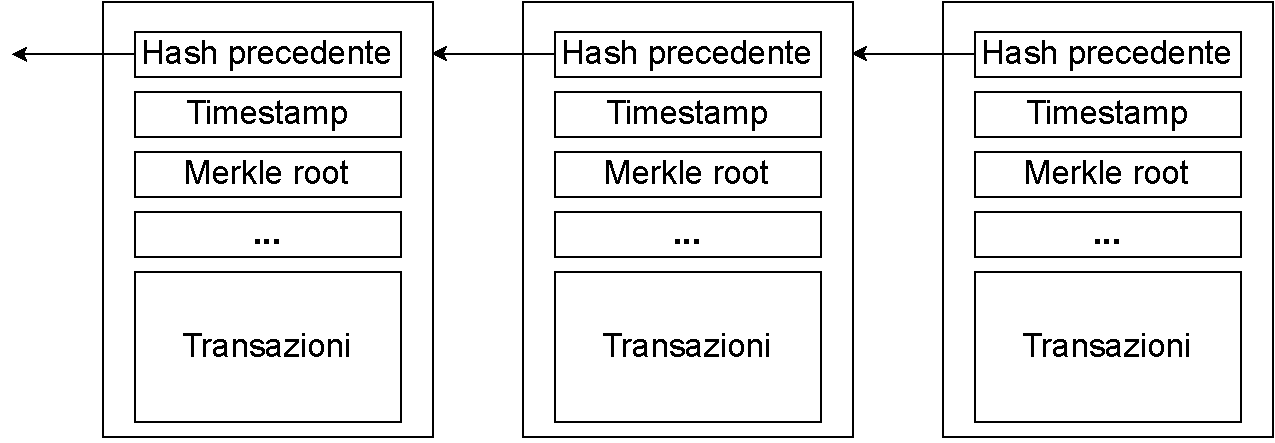
\includegraphics[scale=0.6]{Images/blockChaining.pdf}
    \caption{Schema della Blockchain}
    \label{fig:blockchain}
\end{figure}
\FloatBarrier
\section{Blockchain}
Un generico blocco $B_i$ all’interno della blockchain contiene la sequenza di transazioni relative ad un certo periodo temporale (supponiamo che esse siano n: $T_1$ , $T_2$ , ... ,$T_n$ ) e un valore hash $h_{i-1}$ identificativo del blocco precedente nella catena, che è l’output di una funzione hash crittografica.

È inoltre presente un campo detto nonce, che è il risultato dell’operazione di mining, ovvero del procedimento che porta all’aggiunta di un nuovo blocco alla blockchain. Sono presenti anche altri dati all’interno del blocco, ma al fine di descrivere il meccanismo crittografico che salvaguarda l’integrità della struttura riteniamo sufficiente questo livello di dettaglio è sufficiente.

La Figura \ref{fig:blocchi} mostra la struttura di un generico blocco $B_i$ all’interno della blockchain.
\begin{figure}[h!]
    \centering
    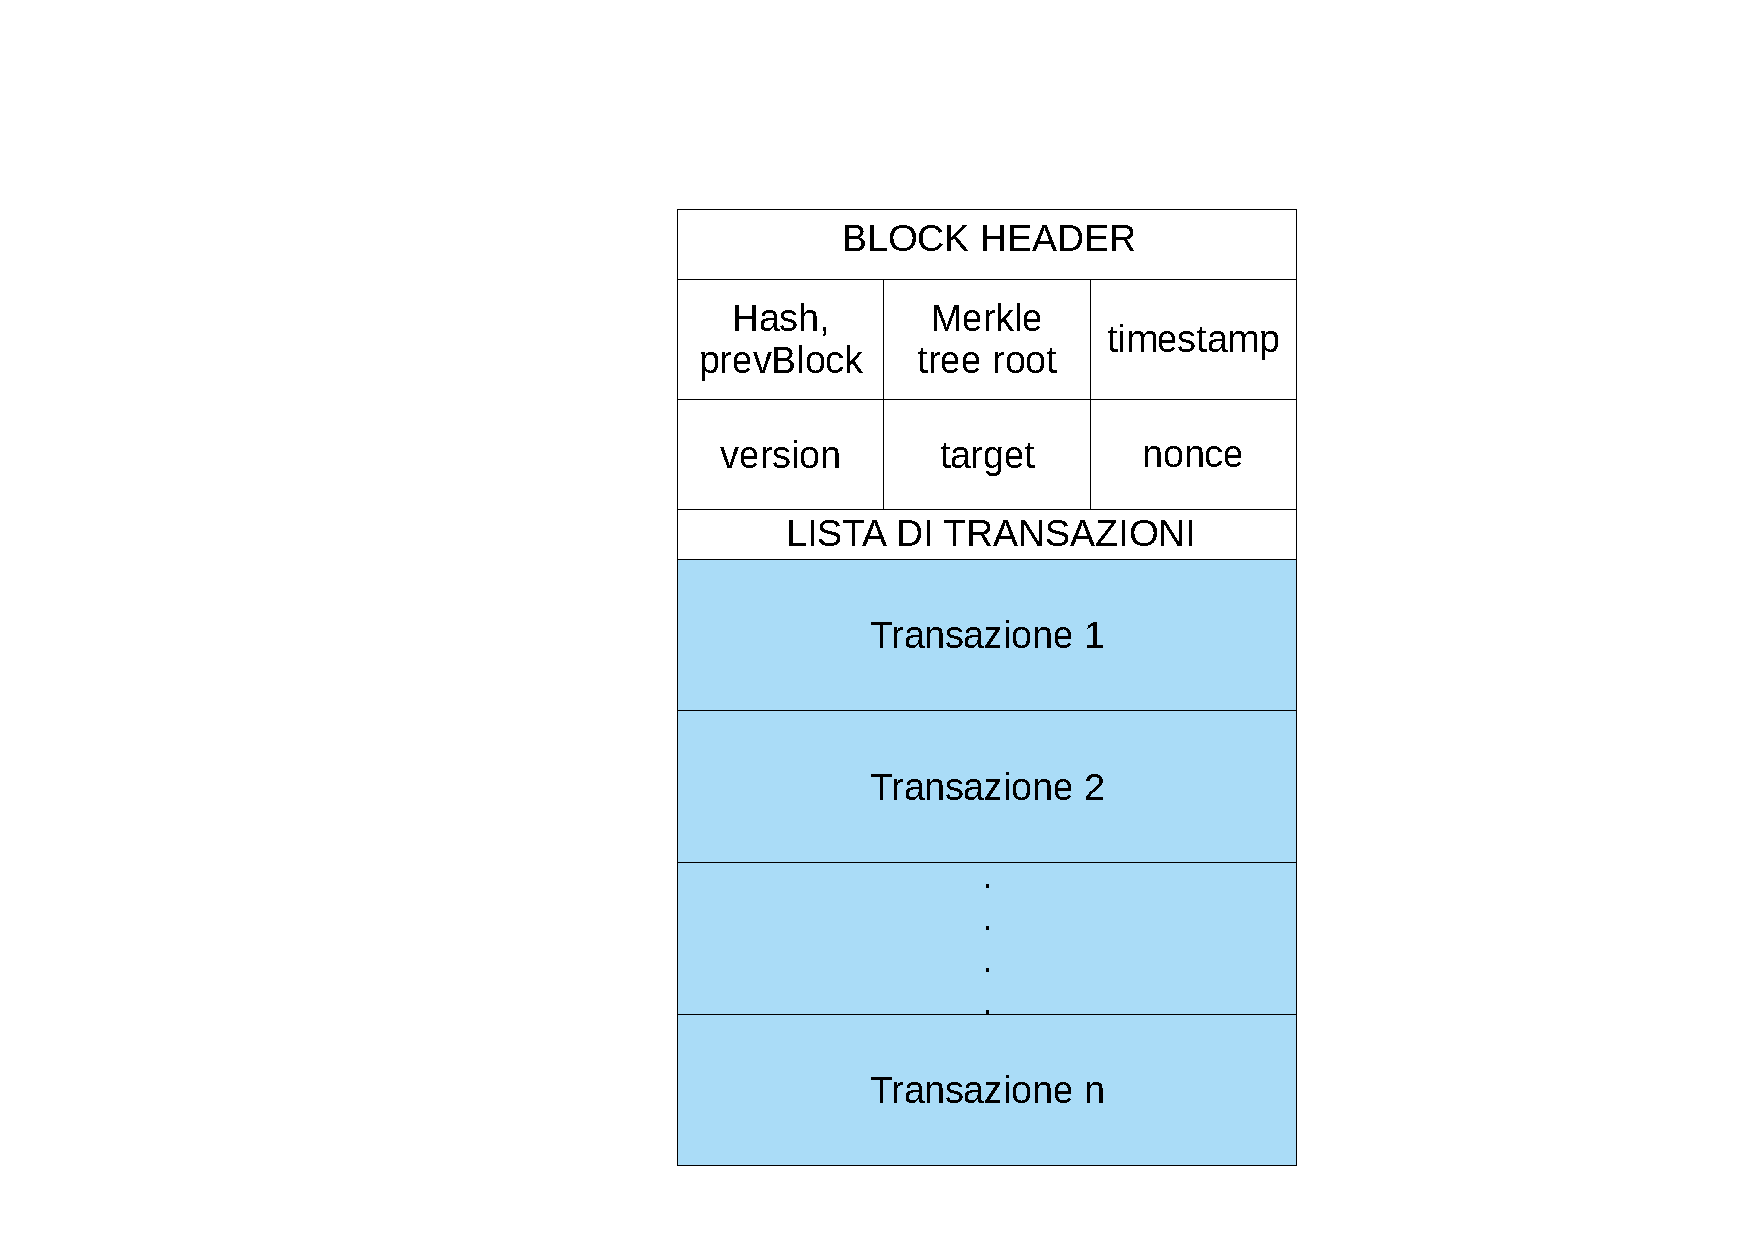
\includegraphics[scale=0.4, trim = 0cm 0cm 0cm 3cm, clip]{Images/blocco_singolo.pdf}
    \caption{Schema di un generico blocco}
    \label{fig:blocchi}
\end{figure}
\FloatBarrier
Come accennato sopra, ogni blocco ha un suo identificativo univoco, una sorta di impronta digitale personale, che è l’output di una opportuna funzione hash.

Un insieme di funzioni hash crittografiche ampiamente usate è quello delle SHA (Secure Hash Algorithm). Una di queste è la SHA-256, funzione hash crittografica che da input di dimensioni variabili produce un fingerprint della lunghezza fissa di 256 bit, ed è la funzione utilizzata per calcolare gli hash dei blocchi all’interno della blockchain di Bitcoin.

L’immagine hash del blocco $B_i$ è calcolata applicando la SHA-256 all’input formato dalla concatenazione delle transazioni contenute in $B_i$ con l'header del blocco, che atraiamo rappresentando i due campi più importanti ovvero il nonce e l'hash del blocco precedente, come riassunto dalla figura \ref{fig:sha-256}:
\begin{figure}[h!]
    \centering
    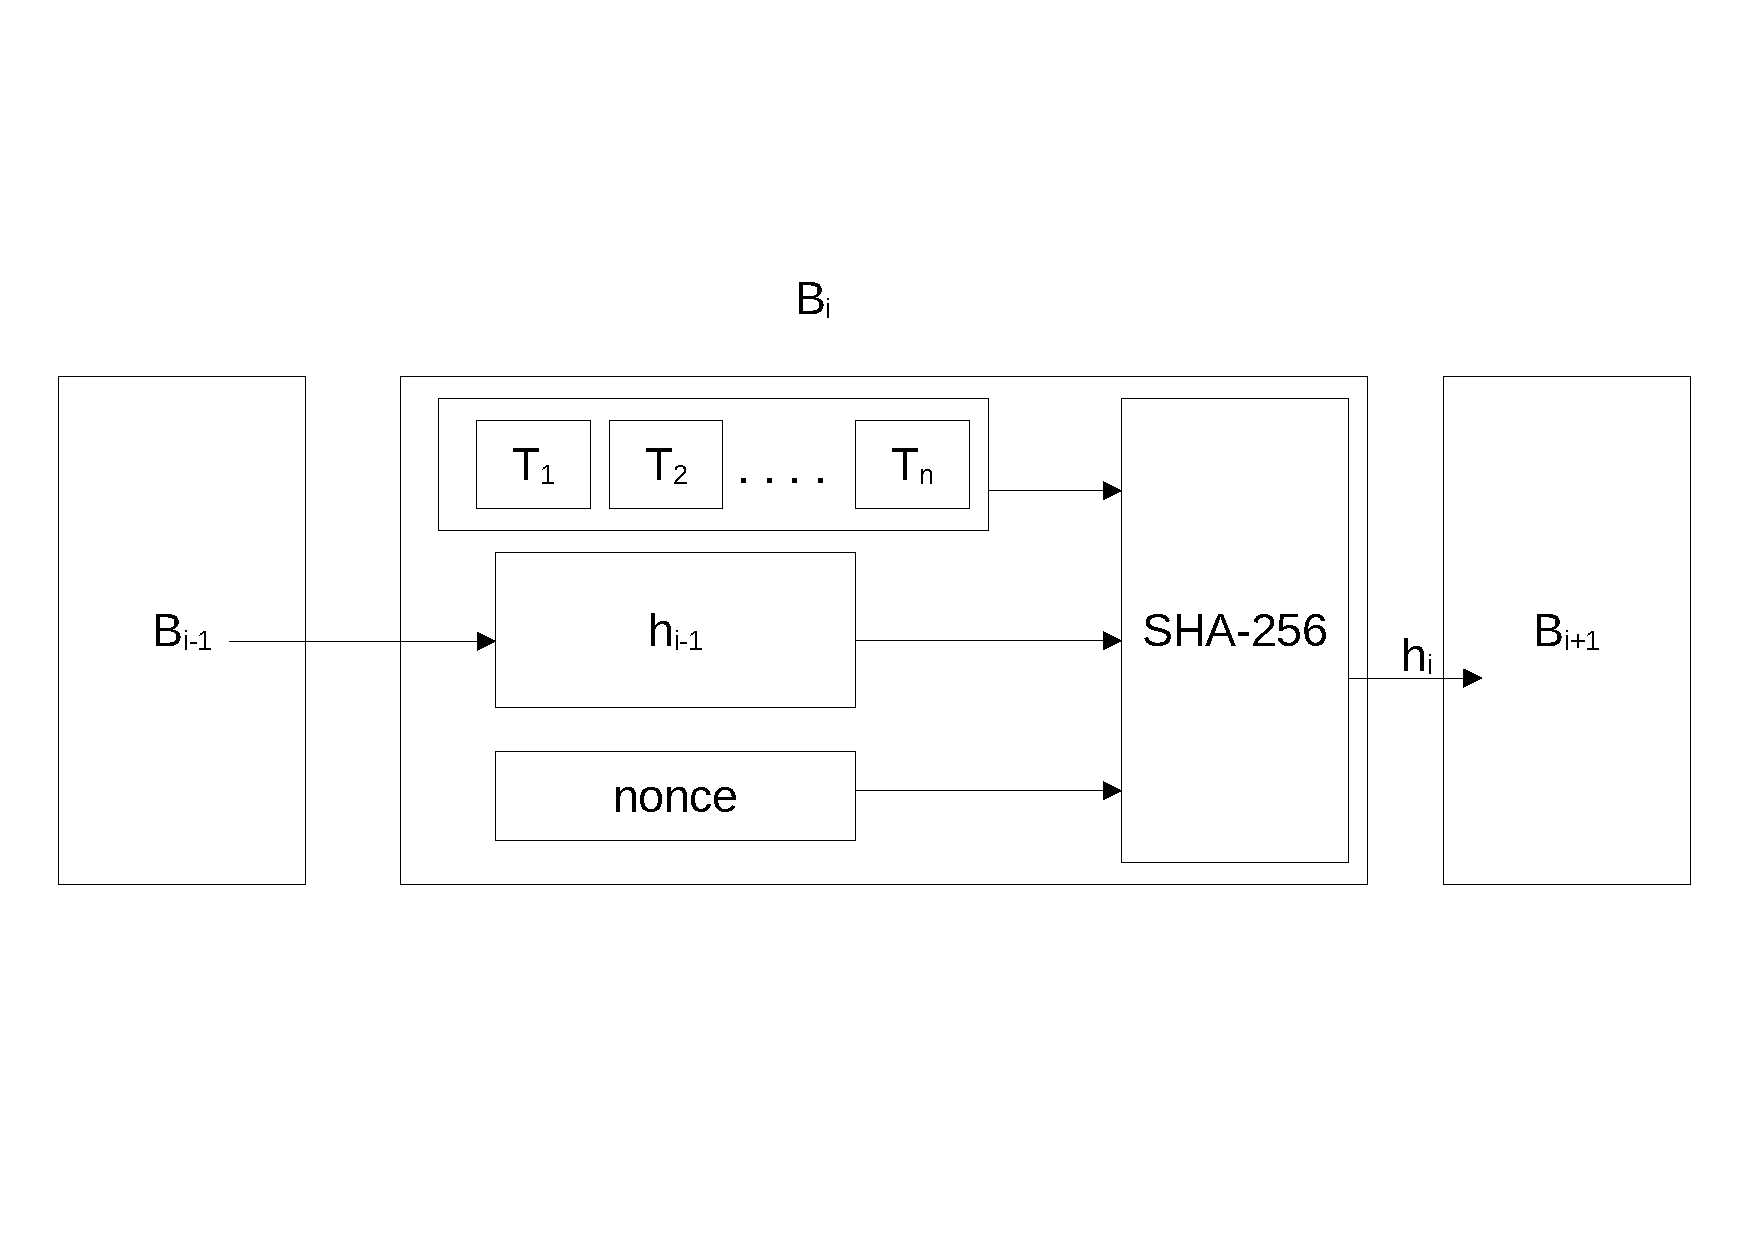
\includegraphics[scale=0.4, trim = 1cm 4cm 0cm 4cm, clip]{Images/blocchi_sha.pdf}
    \caption{Calcolo hash blocco $B_i$}
    \label{fig:sha-256}
\end{figure}
\FloatBarrier
Mentre le transazioni sono note nel blocco, così come è noto l’hash proveniente dal blocco precedente, il valore del nonce è incognito. L’attività di mining consiste nel risolvere un puzzle crittografico: trovare il valore del nonce tale che l’immagine hash prodotta dalla SHA-256 inizi esattamente con $t$ zeri, dove $t$ è un valore prefissato dal sistema, e variabile nel tempo.

La ricerca del nonce per la corretta aggiunta di un blocco è denominata \textbf{Proof of work}. L'unico modo per di trovare il nonce che produca un fingerprint che inizi con $t$ zeri, è quello di applicare ripetutamente la funzione SHA-256 con nonce via via diversi, finchè non si giunge ad un hash che soddisfa la proprietà desiderata. La risoluzione del problema è esponenziale in $t$, infatti la ricerca del nonce richiede tempo $O(2^t)$, ciò rende il problema di difficile risoluzione, in quanto è necessario far eseguire una serie di calcoli computazionalmente pesanti; Il valore di t viene aggiornato periodicamente dal sistema, in modo che la validazione di un blocco richieda sempre in media circa 10/15 minuti di tempo. Negli anni i calcolatori sono stati ottimizzati a livello hardware con lo scopo di calcolare il più rapidamente possibile la funzione SHA-256.

Questo sistema evita che i blocchi già inseriti possano essere modificati retroattivamente: cambiando il contenuto di un blocco, ne cambierebbe anche il valore hash, e ciò implica il dover ricalcolare tutti i nonce dei blocchi successivi ad esso, perchè altrimenti le immagini hash non corrisponderebbero più tra blocchi consecutivi; dunque ciò che è stato scritto sulla blockchain è da considerarsi immutabile, a meno di rendere inconsistente tutta la struttura anche alterandone una sola transazione.

I miner, ossia i nodi della rete che dispongono di nodi di elaborazione abbastanza potenti da risolvere le Proof of Work, rappresentano di fatto gli unici a poter avere il diritto di aggiungere transazioni alla blockchain, e nel farlo consumano un gran quantitativo di energia e di risorse di calcolo; per questo, il primo miner che riesce ad agganciare correttamente un blocco alla blockchain riceve un premio in bitcoin, nella forma di una transazione priva di input e con output l’address del miner: la \textbf{coinbase}, registrata anch’essa nella blockchain come una normale transazione. Il premio, di 25 bitcoin nel 2014, viene dimezzato approssimativamente ogni quattro anni per essere definitivamente azzerato nel 2140 quando il numero complessivo di bitcoin esistenti dovrebbe raggiungere 21 milioni.
\section{Transazioni e Address in Bitcoin}\label{Transazioni}
In questo  paragrafo verranno approfonditi i concetti stessi di transazione e di address, descrivendo con un grado di dettaglio funzionale ai nostri scopi il protocollo di pagamento e, anche in questo caso, la crittografia che ne è alla base, sia per la generazione degli address che per il protocollo di transazione.

I software wallet di bitcoin, per esempio Samurai Wallet, sono caricati sul PC o sullo smartphone di ogni utente A e genera anzitutto una coppia di chiavi privata-pubblica $k_A [prv]$, $k_A [pub]$ per un cifrario asimmetrico su curve ellittiche \cite{curve}.

La chiave privata $k_A [prv]$ è ovviamente nota solo ad A e, come vedremo in seguito, è utilizzata da esso per firmare le transazioni che genera e diffonde sulla rete. La chiave pubblica $k_A [pub]$ è utilizzata per controllare la firma di A ed è anche impiegata come suo identificatore: a tale scopo viene trasformata attraverso applicazioni ripetute della funzione hash SHA-256 (immagine a 256 bit), per essere poi compressa via RIPEMD-160 in un’immagine di 160 bit in testa alla quale è aggiunta una speciale sequenza che indica che la stringa complessiva è di fatto un indirizzo bitcoin.
\begin{figure}[h!]
    \centering
    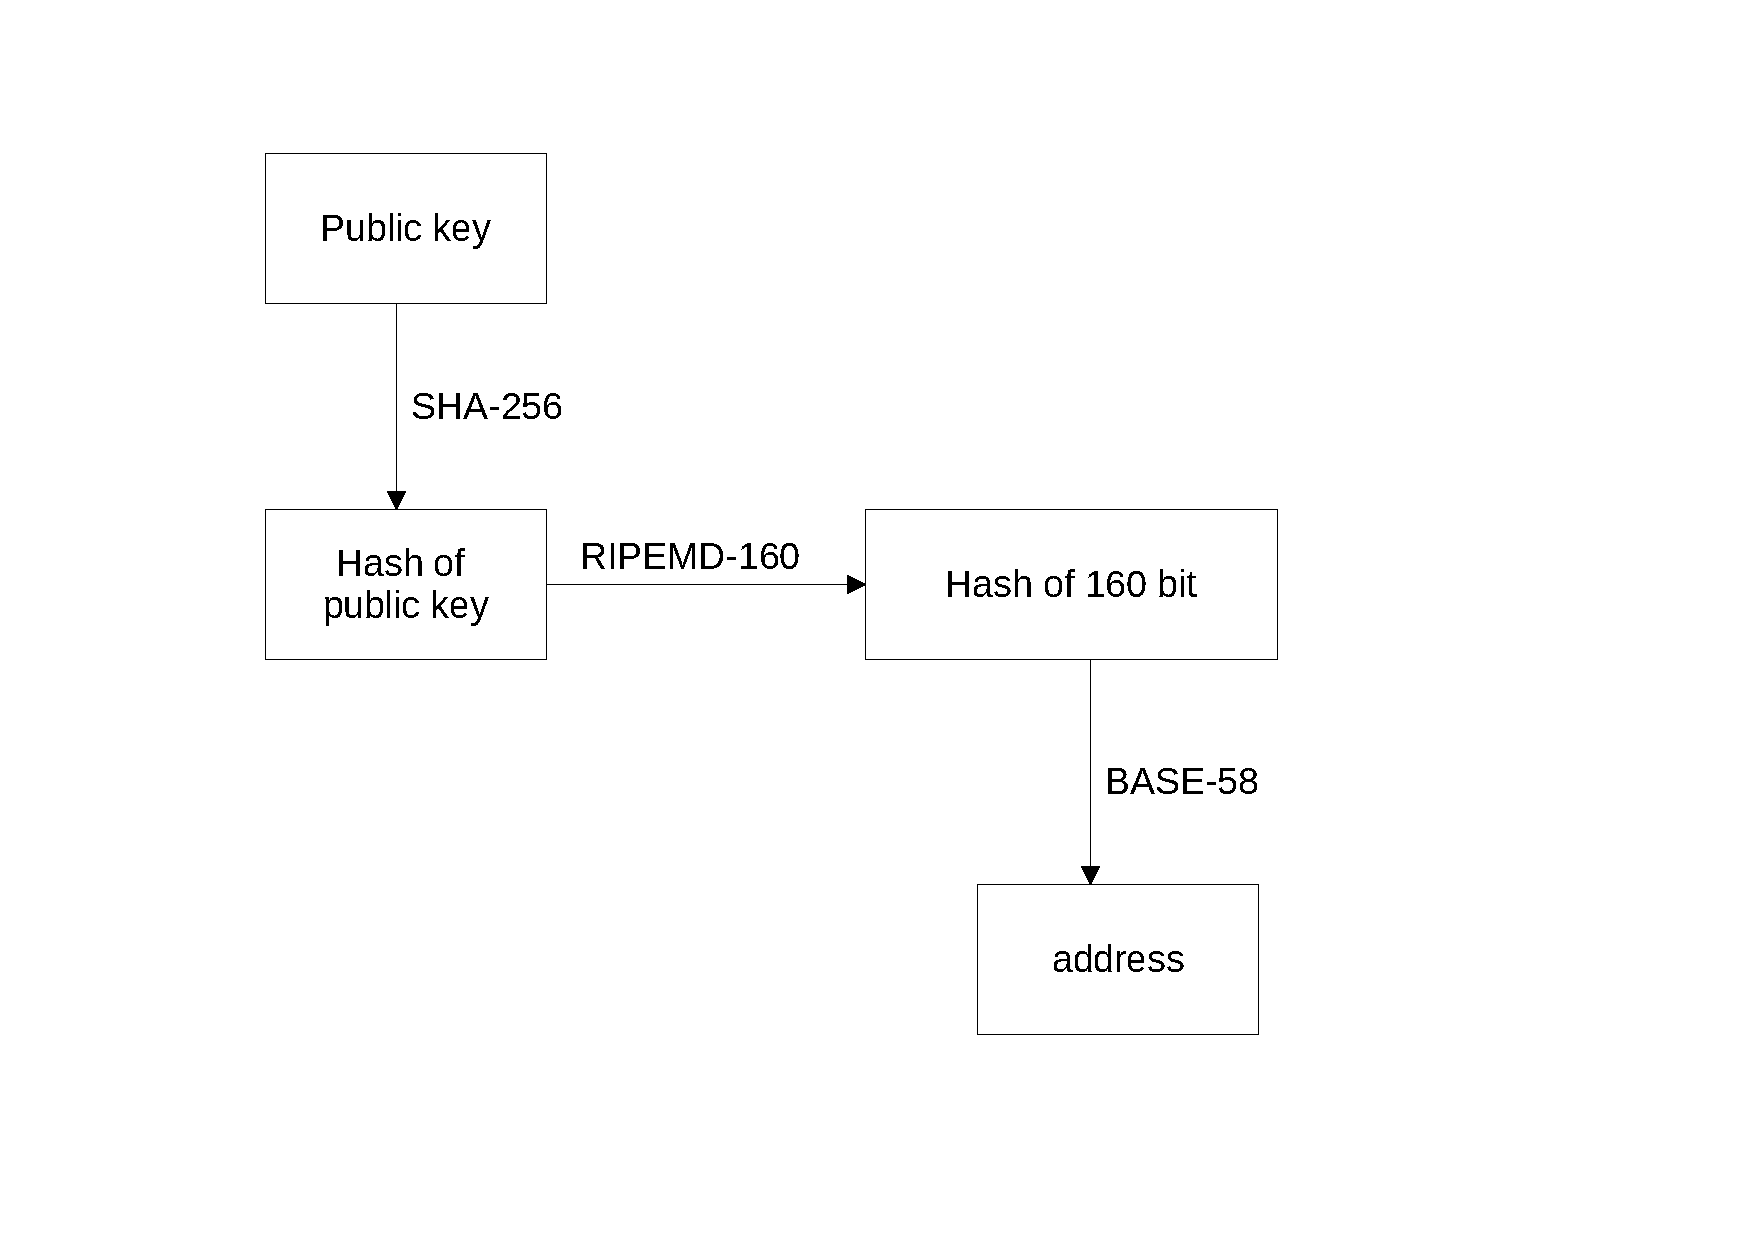
\includegraphics[scale=0.5, trim = 1cm 2cm 0cm 2cm, clip]{Images/address_gen.pdf}
    \caption{Generazione address in Bitcoin}
    \label{fig:sha-256_address}
\end{figure}
\FloatBarrier
Gli address in Bitcoin si presentano quindi come stringhe alfanumeriche di questo tipo: 1BAFWQhH9pNkz3mZDQ1tWrtKkSHVCkc3fV.

Come già osservato questo indirizzo non corrisponde a una “locazione” dell'utente ma a un modo per identificarlo per potergli inviare una transazione. L'insieme delle coppie chiave pubblica-privata è contenuto all'interno di un apposito wallet, ad ognuna di queste coppie è associata un indirizzo però nessuno è a conoscenza del fatto che questi indirizzi appartengano allo stesso wallet.

Questo è importante perchè nonostante un wallet possa avere più address nessuno è a conoscenza che questi address appartengano al medesimo wallet; e possibile tracciare l’attività dei singoli address ma non l’attività di un intero wallet, garantendo un maggiore anonimato. Oltre a creare le chiavi e gli indirizzi il software cliente permette di costruire le transazioni.

Una transazione in Bitcoin può essere riassunta come “il mittente A vuole inviare X bitcoin al ricevente B”, completata dalla firma digitale di A. Si noti che A e B sono indicati attraverso i loro indirizzi Bitcoin e la transazione viene inviata per broadcast a tutti gli utenti. Diversamente da ogni altra forma di transazione economica, il ricevente B non ha la garanzia che la transazione sia valida finché, come vedremo, essa non è convalidata dalla rete. 

In effetti B sarebbe in grado di verificare sia la firma di A che i fondi che A ha a disposizione, poiché la chiave pubblica di A è nota e tutte le transazioni eseguite sulla rete sono pubbliche, ma non ha la possibilità di verificare che A non abbia utilizzato gli stessi fondi in istanti immediatamente precedenti per pagamenti diversi. Formalmente una transazione è innescata secondo il seguente schema:
\begin{center}
\textbf{Protocollo Bitcoin}:
\begin{enumerate}
    \item L’utente A genera un messaggio m = $adr_A$ $-$ X $-$ $adr_B$ , dove $adr_A$ , $adr_B$ sono gli indirizzi Bitcoin di A e B, e X è la somma da trasferire da A a B.
    \item L’utente A calcola l’hash $h = SHA256(m)$ del messaggio e genera la firma $f = D(h, k_A [prv])$ per m.
    \item La coppia $<m, f>$ viene diffusa in broadcast da A sulla rete.
    \item L’utente B attende che la rete convalidi la transazione prima di accettarla.
\end{enumerate}
\end{center}

La chiave privata è l’unico strumento valido per dimostrare la proprietà in bitcoin di un utente A.
La perdita della chiave comporta la perdita della proprietà a causa dell’impossibilità di firmare transazioni, e il furto della chiave da parte di un truffatore che la usi per firmare al posto di A comporta anch’esso la perdita di proprietà.

Un address acquisisce valore in base a quanti bitcoin detiene; quando si usa un address per pagare bitcoin (come input di una transazione), il suo valore viene azzerato, non è possibile spendere solo parte dei bitcoin che costituiscono il valore dell’address. Se un address A paga X bitcoin ad un address B, dopo la transazione il valore di A sarà azzerato, mentre il valore di B aumenterà di X bitcoin. In caso di eventuale resto, nel wallet del pagante si creerà un \textbf{change address}, che acquisirà un valore pari al resto ricevuto.

Il change address può essere un address diverso da A, oppure A stesso, a discrezione dell’utente: per rafforzare l’anonimato è estremamente consigliabile da parte del pagante, al fine di ricevere i resti, utilizzare sempre address diversi da quelli usati per effettuare il pagamento.

Quindi, come mostrato in \ref{fig:transaction}, gli input di una transazione sono precedenti output di un'altra transazione. Gli output di una transazione possono essere in due stati:
\begin{enumerate}
    \item \textbf{speso}: output che compare come input di una transazione successiva;
    \item \textbf{non-speso}: output che non sono input di alcuna transazione.
\end{enumerate}
\begin{figure}[h!]
    \centering
    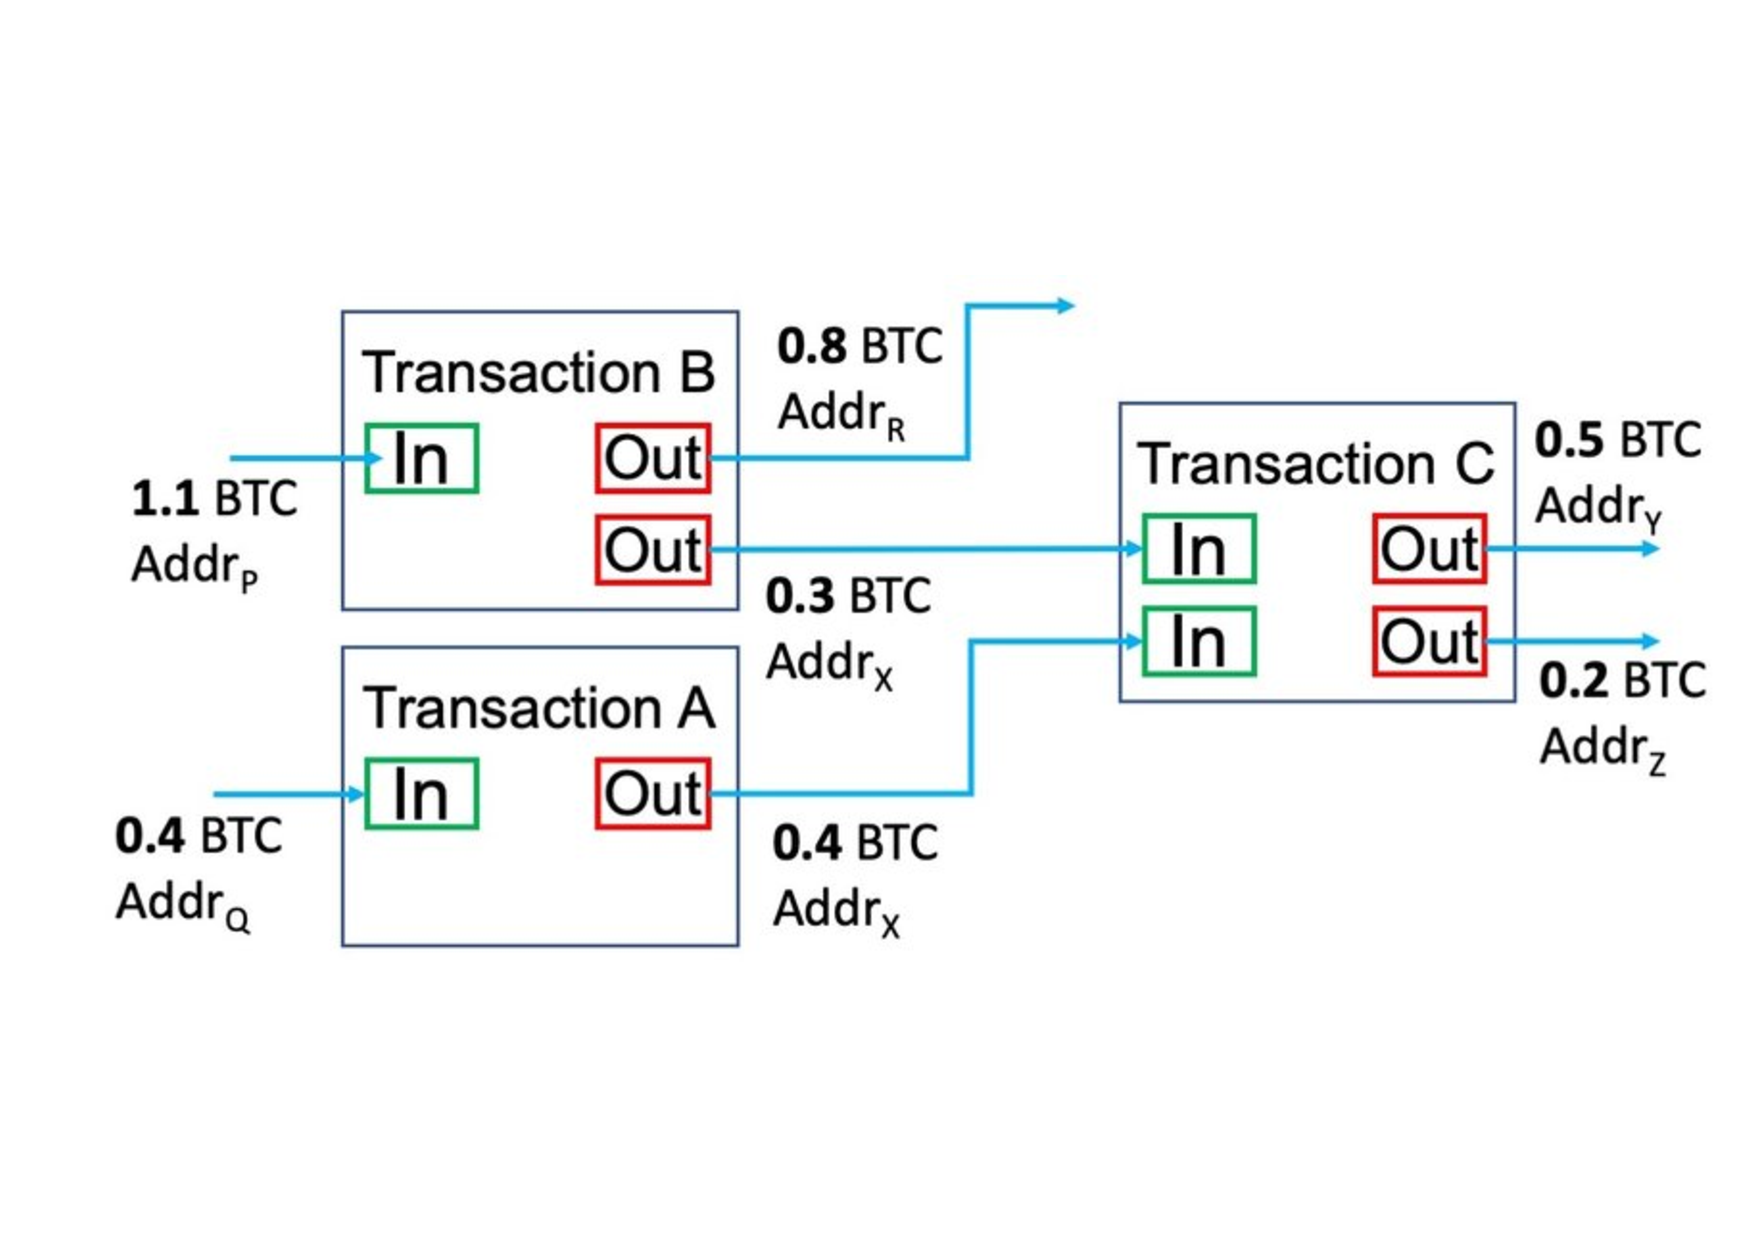
\includegraphics[scale=0.4, trim = 1cm 2cm 0cm 3cm, clip]{Images/Transactions-input-and-output-in-blockchain.jpg.pdf}
    \caption{Transazioni in Bitcoin}
    \label{fig:transaction}
\end{figure}
\FloatBarrier

Tutti gli output non-spesi vengono salvati in un unico insieme denominato UTXO(Unspent Transaction Output) set \cite{utxo}.

L'UTXO set è il sottoinsieme degli output delle transazioni Bitcoin che non sono stati spesi e che possono essere utilizzati come input di altre transazioni. Ogni volta che viene creata una nuova transazione, vengono eliminati output dall'UTXO set poichè passano dallo stato non-speso allo stato speso, inoltre vengono inseriti nuovi UTXO poichè ogni transazione genera almeno un output. Fondamentalmente, le transazioni consumano UTXO (nei loro input) e ne generano di nuovi (nei loro output). Poiché l'UTXO set contiene tutti gli output non spesi, memorizza tutte le informazioni richieste per convalidare una nuova transazione senza dover ispezionare l'intera blockchain. Come suggerisce già il nome, gli UTXO sono effettivamente output di Bitcoin e, come tali, sono costituiti da due parti: l'importo trasferito all'output e lo script che specifica le condizioni da soddisfare per spendere l'output. 

Il vantaggio principale di utilizzare l'UTXO set è la dimensione molto più ridotta dell'intero database delle transazioni (la blockchain), può essere qundi conservato nella RAM, il che velocizza il controllo di validità delle transazioni. L'algoritmo \ref{alg:tx_btc} schematizza la politica di accettazione locale di una transazione. La transazione, accettata localmente eseguendo questo algoritmo può non essere globalmente validata; vengono aggiunte alla blockchain una quando vengono confermate a livello globale.
\begin{algorithm}
\begin{algorithmic}
\State $tx \gets$ ricevi transazione
\For{input $i$ in $tx$}
    \If{($i$ not in local UTXO $or$ firma non valida)} 
        \State scarta $tx$ e fermati
    \EndIf
\EndFor
\If{sum(inputs) $<$ sum(outputs)}
    \State scarta $tx$ e fermati
\EndIf
\For{input $i$ in $tx$}
    \State rimuovi $i$ dall'UTXO set locale
\EndFor
\State inoltra $tx$
\end{algorithmic}
\caption{Gestione transazione Bitcoin}
\label{alg:tx_btc}
\end{algorithm}
\FloatBarrier
In Bitcoin quindi non esiste un saldo memorizzato, il bilancio di un address infatti è un costrutto derivato dai Software Wallet. Il wallet calcola il saldo di un address scansionando la blockchain e sommando gli importi di tutti gli UTXO relativi a quel singolo address. Infatti se un address riceve diversi importi, questi non vengono aggregati ma vengono tutti salvati all'interno dell'UTXO set. Il bilancio complessivo di un wallet invece non è altro che la somma dei bilanci dei singoli address appartenenti a quel wallet. 
Gli utenti non conoscono il saldo complessivo di un utente proprio perchè non sanno quali address appartengano ad un determinato wallet, esistono tuttavia delle tecniche e delle euristiche che permettono non solo di conoscere gli address di un wallet ma consentono anche di conoscere le informazioni personali del proprietario.
\section{Anonimato in Bitcoin}\label{Anonimato}
L'anonimato in Bitcoin dovrebbe garantire che sia impossibile collegare address differenti, ovvero capire che appartengano ad uno stesso utente, e che non sia possibile scoprire l'identità di un proprietario di un wallet.

Nel protocollo Bitcoin l'anonimato però è garantito solo attraverso lo pseudonimo, ogni utente invia e spende bitcoin tramite un numero arbitrario di address che non contengono informazioni reali sull'utente; per questo Bitcoin non viene definito anonimo ma pseudo-anonimo; esistono infatti diversi attacchi che permettono di violare l'anonimato di Bitcoin \cite{de-anonimizzazione} \cite{de-anon2}.

Uno di questi attacchi si basa sull'analisi delle transazioni salvate sulla blockchain che, come ricordiamo, è pubblica e immutabile. Lo scopo di questo attacco è di aggregare address differenti in cluster, ciascuno rappresentante un singolo utente, utilizzando le informazioni memorizzate nella blockchain. Una volta ottenuti questi cluster è poi possibile utilizzare informazioni esterne per identificare il proprietario di un singolo cluster. 

Per formare questi cluster vengono utilizzate delle euristiche basate sul comportamento degli utenti di Bitcoin, queste regole quindi dipendono dal tempo e non sono assolute. 

Le due euristiche più utilizzate sono:
\begin{enumerate}
    \item \textbf{inputs multipli};
    \item \textbf{change address}.
\end{enumerate}

La prima euristica dice:
\begin{center}
    ``\textit{In una transazione multi-input tutti gli address appartengono allo stesso utente}"
\end{center}

Ogni transazione deve essere firmata per ogni input, significa che per firmare la transazione la chiave privata di ciascun input dovrebbe essere nota. Ciò implica che il firmatario conosca tutte le chiavi private e quindi è il proprietario di tutti gli indirizzi di input. Questa prima semplice euristica è stata utilizzata con successo in passato ma non è più valida per tutte le transazioni. La prima contromisura proposta è stata CoinJoin \cite{coinjoin} nel 2013, l'idea principale è che un insieme di utenti si incontri e crei collettivamente una singola transazione utilizzando i loro address. Questa situazione quindi porterebbe ad un falso positivo della regola euristica appena enunciata, infatti gli address di input non appartengono ad un unico utente.

La seconda euristica dice: 
\begin{center}
    ``\textit{il change address appartiene allo stesso proprietario degli address di input}"
\end{center}

Il problema principale di questa regola è capire quali degli address di output sia il change address, escludendo il caso di ''self change", ovvero quando il change address è uno degli address di input. 

Un address $a$ viene definito change address sse:
\begin{itemize}
    \item la transazione non è coinbase;
    \item è presente più di un output;
    \item negli address di output non è presente alcun address di input(niente ''self change");
    \item è la prima volta che $a$ appare nella blockchain e non ci sono altri address di output che soddisfano questa condizione.
\end{itemize}

L'attacco che verrà analizzato in questa tesi, denominato \textbf{Dust Attack}, basa la propria strategia sulla prima euristica, in particolare l'attaccante agisce in modo che le vittime generino transazioni multi-input così da poter formare un cluster di address appartenenti ad un unico utente.






